% The step function of both SPARX-128/128 and SPARX-128/256

\begin{figure}
    \begin{subfigure}{0.7\textwidth}
        \begin{center}
            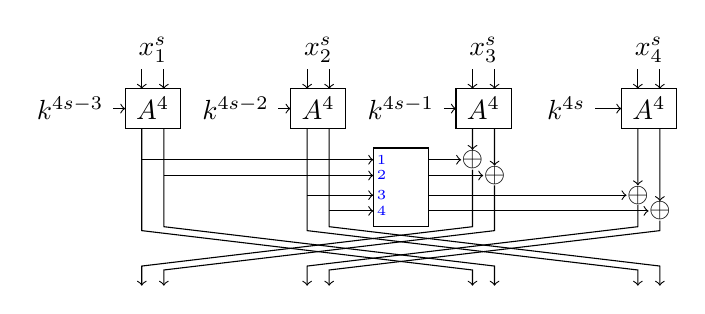
\begin{tikzpicture}[xscale=0.7, yscale=0.5]
                %% input
                \draw (-4.5, +5.0) node(x0){$x^s_1$} ;
                \draw (-1.5, +5.0) node(x1){$x^s_2$} ;
                \draw (+1.5, +5.0) node(x2){$x^s_3$} ;
                \draw (+4.5, +5.0) node(x3){$x^s_4$} ;
                \draw[->] (-4.7, +4.5) -- (-4.7, +4.0) ;
                \draw[->] (-4.3, +4.5) -- (-4.3, +4.0) ;
                \draw[->] (-1.7, +4.5) -- (-1.7, +4.0) ;
                \draw[->] (-1.3, +4.5) -- (-1.3, +4.0) ;
                \draw[->] (+1.7, +4.5) -- (+1.7, +4.0) ;
                \draw[->] (+1.3, +4.5) -- (+1.3, +4.0) ;
                \draw[->] (+4.7, +4.5) -- (+4.7, +4.0) ;
                \draw[->] (+4.3, +4.5) -- (+4.3, +4.0) ;
                %% S-Box layer
                \draw (-6.0, +3.5) node(k0){$k^{4s-3}$} ;
                \draw (-3.0, +3.5) node(k1){$k^{4s-2}$} ;
                \draw (+0.0, +3.5) node(k2){$k^{4s-1}$} ;
                \draw (+3.0, +3.5) node(k3){$k^{4s}$} ;
                \draw[->] (k0) -- (-5.0, +3.5) ;
                \draw[->] (k1) -- (-2.0, +3.5) ;
                \draw[->] (k2) -- (+1.0, +3.5) ;
                \draw[->] (k3) -- (+4.0, +3.5) ;
                \draw (-5.0, +3.0) rectangle node[pos=0.5]{$A^4$} (-4.0, +4.0) ;
                \draw (-2.0, +3.0) rectangle node[pos=0.5]{$A^4$} (-1.0, +4.0) ;
                \draw (+1.0, +3.0) rectangle node[pos=0.5]{$A^4$} (+2.0, +4.0) ;
                \draw (+4.0, +3.0) rectangle node[pos=0.5]{$A^4$} (+5.0, +4.0) ;
                %% Linear layer
                \draw (-0.5, +0.5) rectangle node[pos=0.5]{$\Lsixty$} (+0.5, +2.5) ;
                \draw (+1.3, +2.2) node[inner sep=0](xor0){$\oplus$} ;
                \draw (+1.7, +1.8) node[inner sep=0](xor1){$\oplus$} ;
                \draw (+4.3, +1.3) node[inner sep=0](xor2){$\oplus$} ;
                \draw (+4.7, +0.9) node[inner sep=0](xor3){$\oplus$} ;
                % Left to right
                \draw[->] (-4.7, 3.0) -- (-4.7, 0.4) -- (+1.3, -0.6) -- (+1.3, -1.0) ;
                \draw[->] (-4.3, 3.0) -- (-4.3, 0.5) -- (+1.7, -0.5) -- (+1.7, -1.0) ;
                \draw[->] (-1.7, 3.0) -- (-1.7, 0.4) -- (+4.3, -0.6) -- (+4.3, -1.0) ;
                \draw[->] (-1.3, 3.0) -- (-1.3, 0.5) -- (+4.7, -0.5) -- (+4.7, -1.0) ;
                % Right to left
                \draw[->] (+1.3, 3.0) -- (xor0) ;
                \draw[->] (+1.7, 3.0) -- (xor1) ;
                \draw[->] (+4.3, 3.0) -- (xor2) ;
                \draw[->] (+4.7, 3.0) -- (xor3) ;
                \draw[->] (+0.5, 2.2) -- (xor0) ;
                \draw[->] (+0.5, 1.8) -- (xor1) ;
                \draw[->] (+0.5, 1.3) -- (xor2) ;
                \draw[->] (+0.5, 0.9) -- (xor3) ;
                \draw[->] (xor0) -- (+1.3, 0.5) -- (-4.7, -0.5) -- (-4.7, -1.0) ;
                \draw[->] (xor1) -- (+1.7, 0.4) -- (-4.3, -0.6) -- (-4.3, -1.0) ;
                \draw[->] (xor2) -- (+4.3, 0.5) -- (-1.7, -0.5) -- (-1.7, -1.0) ;
                \draw[->] (xor3) -- (+4.7, 0.4) -- (-1.3, -0.6) -- (-1.3, -1.0) ;
                % arrows to L'
                \draw[->] (-4.7, 2.2) -- (-0.5, 2.2) ;
                \draw (-0.35, 2.2) node{\color{blue} \tiny 1} ;
                \draw[->] (-4.3, 1.8) -- (-0.5, 1.8) ;
                \draw (-0.35, 1.8) node{\color{blue} \tiny 2} ;
                \draw[->] (-1.7, 1.3) -- (-0.5, 1.3) ;
                \draw (-0.35, 1.3) node{\color{blue} \tiny 3} ;
                \draw[->] (-1.3, 0.9) -- (-0.5, 0.9) ;
                \draw (-0.35, 0.9) node{\color{blue} \tiny 4} ;
            \end{tikzpicture}
            \caption{\label{fig:sparx-128-step}Step structure.}
        \end{center}
    \end{subfigure}
    \begin{subfigure}{0.27\textwidth}
        \begin{center}
            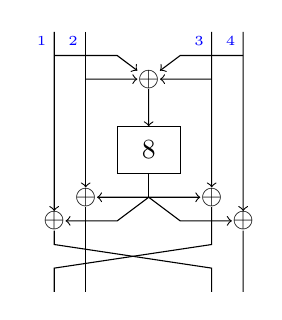
\begin{tikzpicture}[xscale=0.8, yscale=0.6]
                \draw (+1.0, 5.0) node[inner sep=0](xorT){$\oplus$};
                \draw[->] (-0.5, 5.5) -- (+0.5, 5.5) -- (xorT) ;
                \draw[->] (+0.0, 5.0) -- (xorT) ;
                \draw[->] (+2.0, 5.0) -- (xorT) ;
                \draw[->] (+2.5, 5.5) -- (+1.5, 5.5) -- (xorT) ;
                \draw (-0.5, 2.0) node[inner sep=0](xorLL){$\oplus$};
                \draw (+0.0, 2.5) node[inner sep=0](xorL){$\oplus$};
                \draw (+2.0, 2.5) node[inner sep=0](xorR){$\oplus$};
                \draw (+2.5, 2.0) node[inner sep=0](xorRR){$\oplus$};
                \draw[->] (-0.5, 6.0) -- (xorLL) ;
                \draw (xorLL) -- (-0.5, 1.5) -- (+2.0, +1.0) -- (+2.0, +0.5);
                \draw[->] (+0.0, 6.0) -- (xorL) ;
                \draw (xorL) -- (+0.0, 0.5);
                \draw[->] (+2.0, 6.0) -- (xorR) ;
                \draw (xorR) -- (+2.0, 1.5) -- (-0.5, +1.0) -- (-0.5, +0.5);
                \draw[->] (+2.5, 6.0) -- (xorRR) ;
                \draw (xorRR) -- (+2.5, 0.5);
                \draw (+0.5, +3.0) rectangle node[pos=0.5]{$\lll 8$} (+1.5, 4.0) ;
                \draw[->] (xorT) -- (+1.0, +4.0) ;
                \draw (+1.0, +3.0) -- (+1.0, +2.5) ;
                \draw[->] (+1.0, +2.5) -- (+0.5, +2.0) -- (xorLL) ;
                \draw[->] (+1.0, +2.5) -- (xorL) ;
                \draw[->] (+1.0, +2.5) -- (xorR) ;
                \draw[->] (+1.0, +2.5) -- (+1.5, +2.0) -- (xorRR) ;
                % helping numbers
                \draw (-0.7, +5.8) node{\color{blue} \tiny 1} ;
                \draw (-0.2, +5.8) node{\color{blue} \tiny 2} ;
                \draw (+1.8, +5.8) node{\color{blue} \tiny 3} ;
                \draw (+2.3, +5.8) node{\color{blue} \tiny 4} ;
            \end{tikzpicture}
            \caption{\label{fig:sparx-128-L-prime}$\Lsixty$.}
        \end{center}
    \end{subfigure}
    \FigDef{sparx128}{The step structure of \sparxinstance{128}{128} and \sparxinstance{128}{256}.}
\end{figure}